\section{Methods}


\subsection{Project Methodology}
When working in a project it is generally a good idea to work according to a predetermined project methodology model. This tends to make the work more effective and produce better quality. That is, more is produced during the same amount of time, the final product is more thought out, better teamwork etc.

Simply, if you have a plan at the start it is easier to stick to that plan and stay on the same path as intended, rather than shifting to another one. That is not to say that the plan cannot change, but if it does it does so controllably.

A historically good model has been the waterfall model. However, in the software industry this has changed lately with the agile methodology being more popular and has proven to be very effective.

\subsubsection{Agile}
Basically, the agile model says that rather than planning a workload for 6 months forward or so it is better to work in short iterations. These iterations should be between 1 - 4 weeks depending on the team.
Instead of trying to estimate the time it will take to complete an entire project, the team is given a finite time frame and tries to do as much as possible during that time. During this time, the team works very closely to the customer and project owner to make sure that they will get what they want and ask for.
For selecting items to work with for every sprint the team keeps a backlog of item it wishes to complete during the project. Every sprint these items (or stories) are picked out and included into the sprint and estimated in size. The stories themselves should be collected from customers, project owner, users and people connected to the product. This way, the team knows what the purpose is with developing a certain thing. If there is any doubt about a specific feature it should be easier to ask than to assume.

This is of course a simplified version of how the agile method works. 'Extreme Programming Pocket Guide' is a good book for anyone who wants to read more about agile methodology.

\cite{extremeProgramming}


\subsubsection{How we used the agile methodology}
\textbf{Sprints} \\
For our planned work we have decided to work in two week period sprints where we begin on a Tuesday and end on a Monday. At each start of a sprint we pick out stories to focus on for the coming two weeks and try to estimate how long each of them will take.
On weekdays we start with a quick discussion about yesterdays work and what we are planning to do today. This is for everyone to be up to speed about the other persons work.
At the end of the sprint everything is review and analysed so to do even better the next sprint by correcting possible faults.

\textbf{Story board} \\
For organizing our sprints we used a story board which contained an area for our backlog items and four rows for our stories during a sprint. The stories were broken into tasks which were placed on either one of the columns (Started, In Progress, Waiting, Completed).
Each story was estimated with a size which was a number in the fibonacci sequence. Each story was also divided into 5 parts (Started, Halfway done, Completed, Reviewed, Verified). These two numbers were multiplied and summed up with all the other stories to get how many points the sprints had. As we worked these points were subtracted and ultimately hit zero when we were done with everything. We plotted the progress on a chart as well for graphic. This is called a burndown.

\begin{figure}[hbtp]
\begin{center}
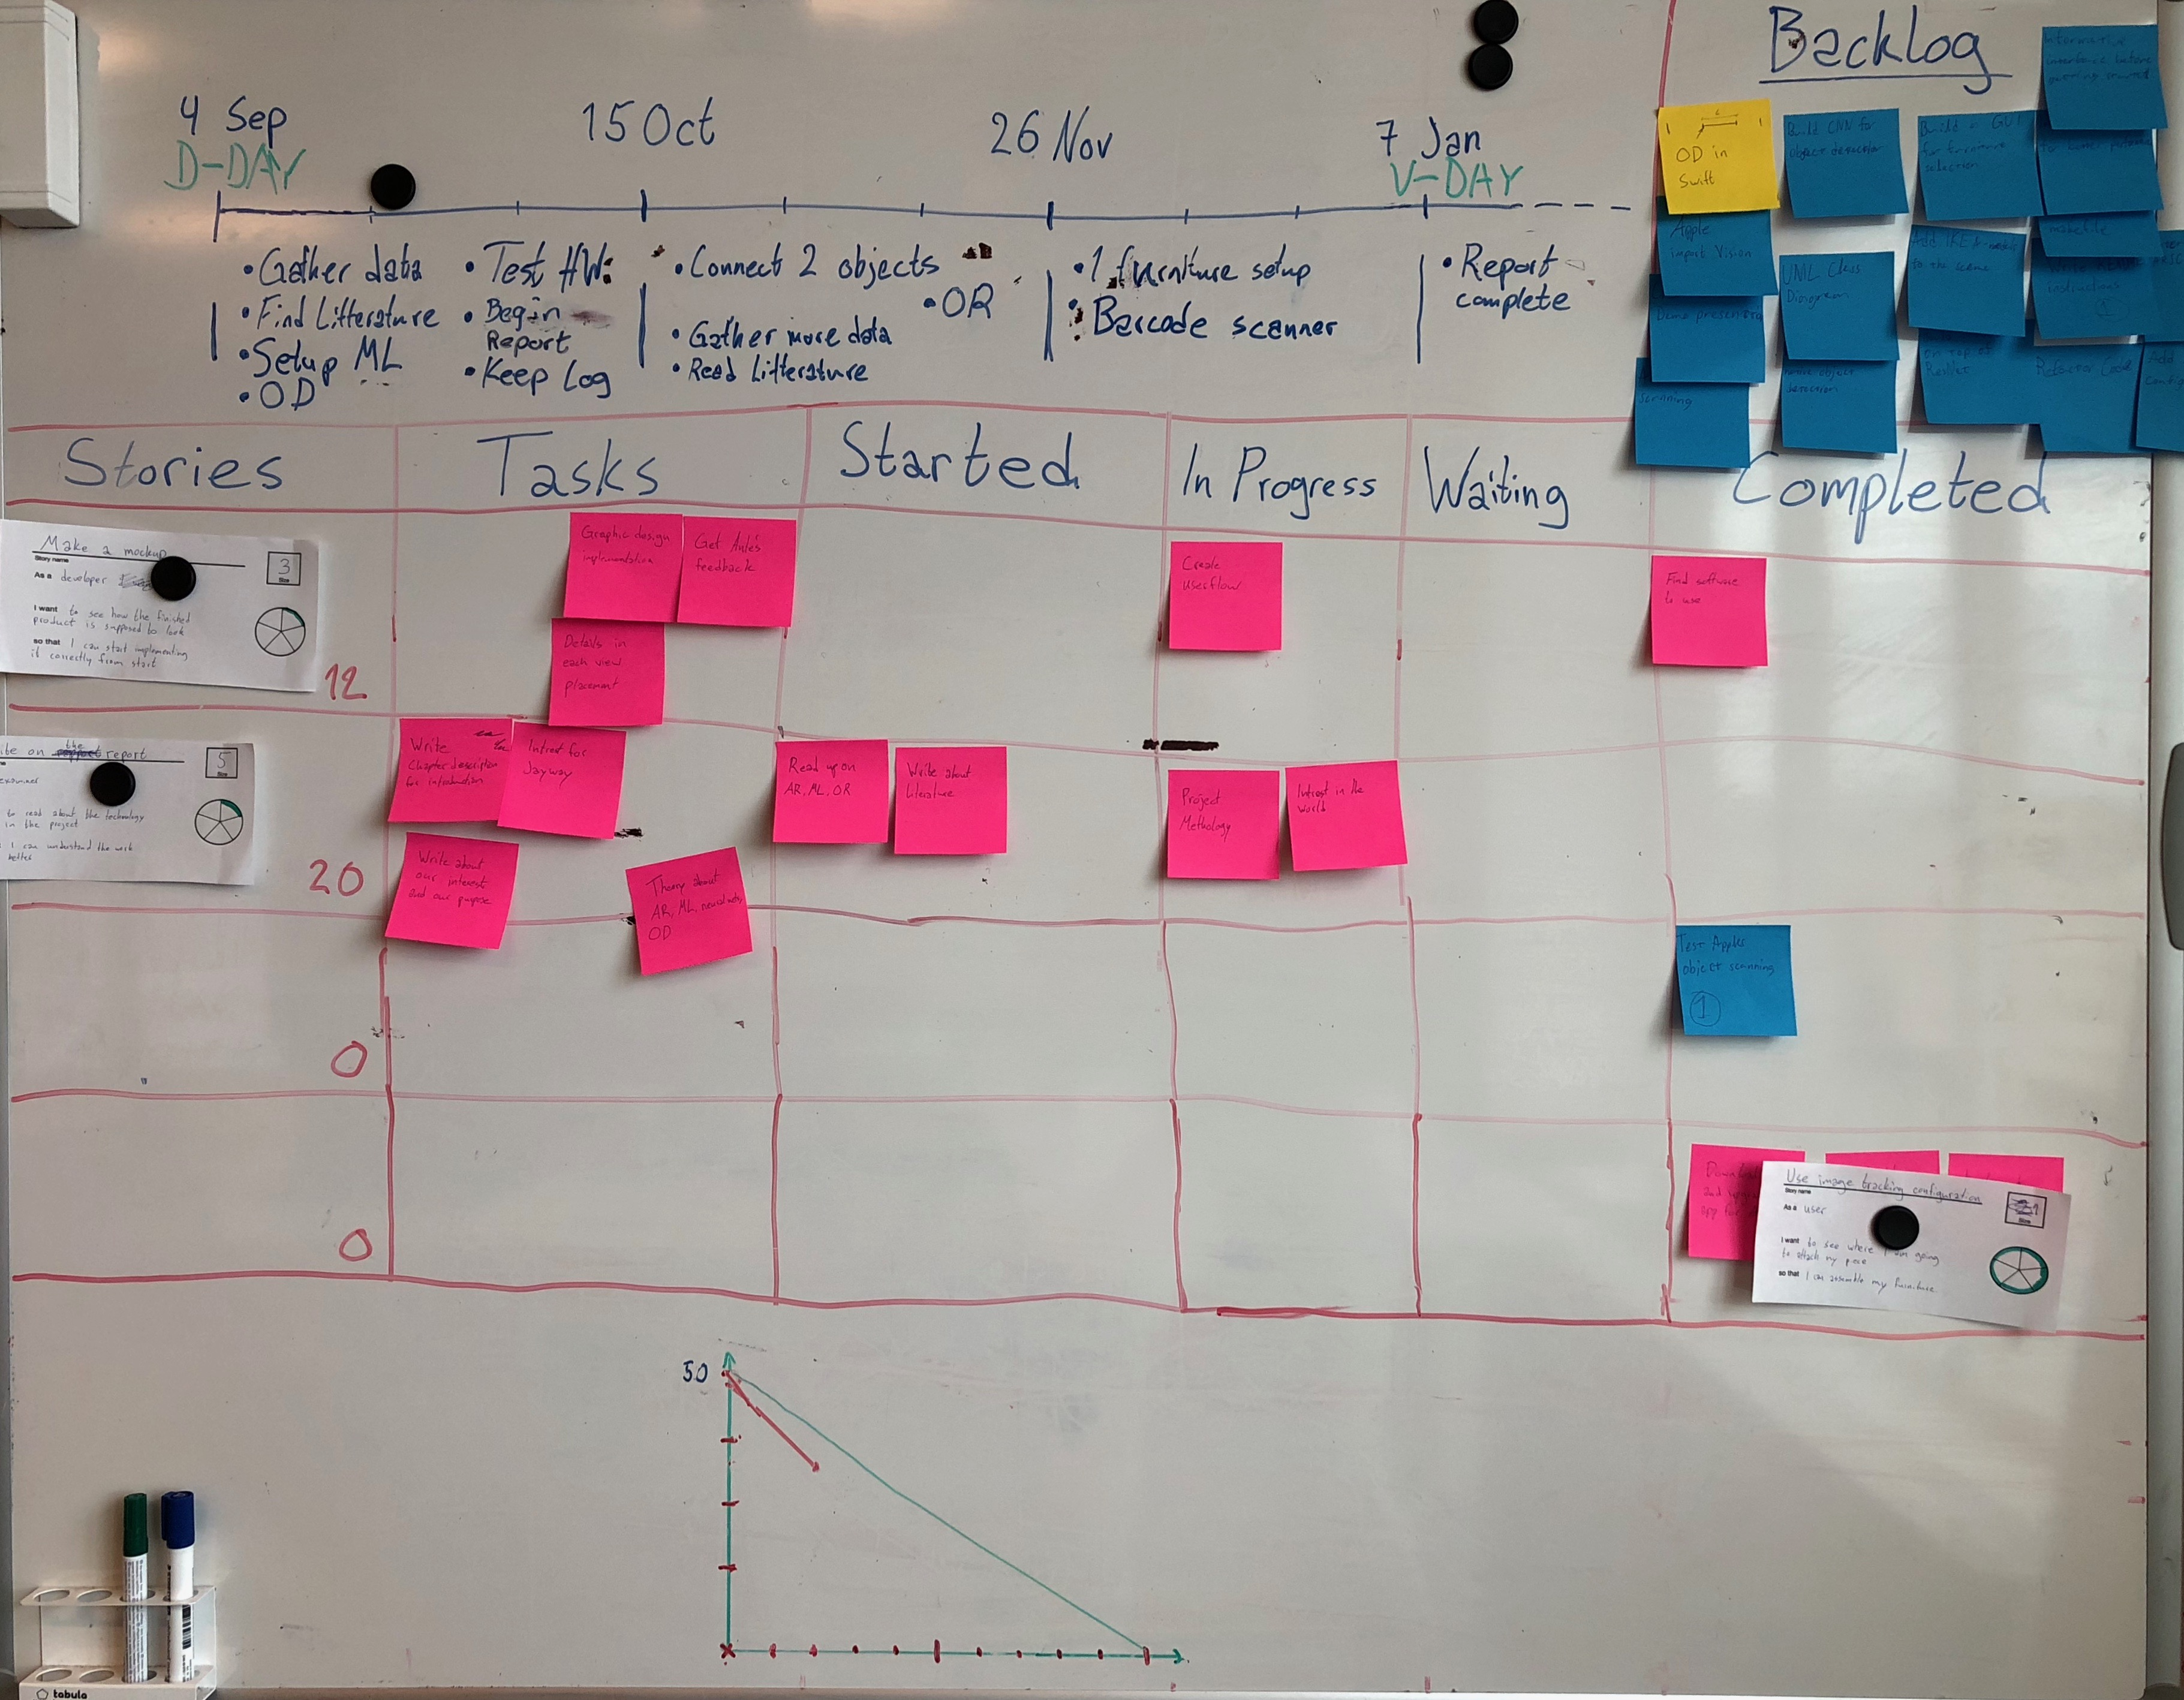
\includegraphics[width = 0.5\textwidth]{./Images/story_board.jpg} 
\caption{Story board used during the project}
\end{center}
\end{figure}


\textbf{Close relationship with project owner} \\
We worked very close to the project owner by sitting on desks right across him. Whenever we had a questing we could simply raise our head and ask it.

\subsection{Matlab prototype for Object Detection}

\subsection{Testing Object Scanning with ARKit2}
Apple's ARKit2 has a feature where it can detect scanned 3D objects. For scanning, they have developed an app that can be downloaded from their website. \cite{ARScanning}
After the scanning is complete the app lets you export the model to then include it in your ARKit2 project. Once in the project it is simply imported into the ARWorldTrackingConfiguration like shown below.

\lstinputlisting[language=swift,firstline=63,lastline=71]{../../Application/ObjectDetectionInAR/ObjectDetectionInAR/ARViewController.swift}

\begin{figure}[hbtp]
\begin{center}
\includegraphics[width = 0.32\textwidth]{./Images/3dscanning1.png}
\includegraphics[width = 0.32\textwidth]{./Images/3dscanning2.png}
\includegraphics[width = 0.32\textwidth]{./Images/3dscanning3.png} 
\caption{3D Scanning using Apple's app. On the right, the bounding box is defined so that no reference points from other objects are included. In the middle, the object is scanned by aiming the camera around the object at all angles. On the right the created model is tested. In this case, the object is detected after 0.4 seconds.}
\end{center}
\end{figure}

Once imported into our project we were able to test the performance of recognizing and tracking three pieces of our furniture.
Sadly, this method came up short for our purpose. When testing live in our app the time for detection were much longer ( over 1 second ) which made tracking them difficult. The tracking wasn't smooth but rather choppy. Many times, the object wasn't detected at all. This was mainly due to our objects being a little big to fit the screen while being close with the camera but also that the object had a lot of empty space within its bounding box.

The detection worked best while being in the same environment, static with the same kind of lightning conditions, but fell short when the object was moving or being held. Therefore, since the user is going to hold the pieces by hand and moving them around, this method cannot be used for our purpose.

\subsection{Testing Object Tracking with Vision package}
Vision is a package from Apple which contains a lot of different methods for images and video. It contains still image analysis, image sequence analysis, object tracking, face detection etc.

On their website, Apple has a project that lets any user try out the object tracking on a video. When trying this on one of the furnitures we are going to assemble, the result was very promising. While the parts were laying on the floor and simultaneously moving the camera around, the objects were tracked fairly well. It was only when the camera was moved in such a way that made the pieces rotate in the picture that it started having a hard time tracking it.

For solving this, object detection can be performed in a reasonable time interval and be tracked until object detection is performed once again etc.

\cite{ObjectTracking}

\subsection{Tensorflow and Machine Learning}

\subsection{AR implementation in ARKit}

\begin{figure}[hbtp]
\begin{center}
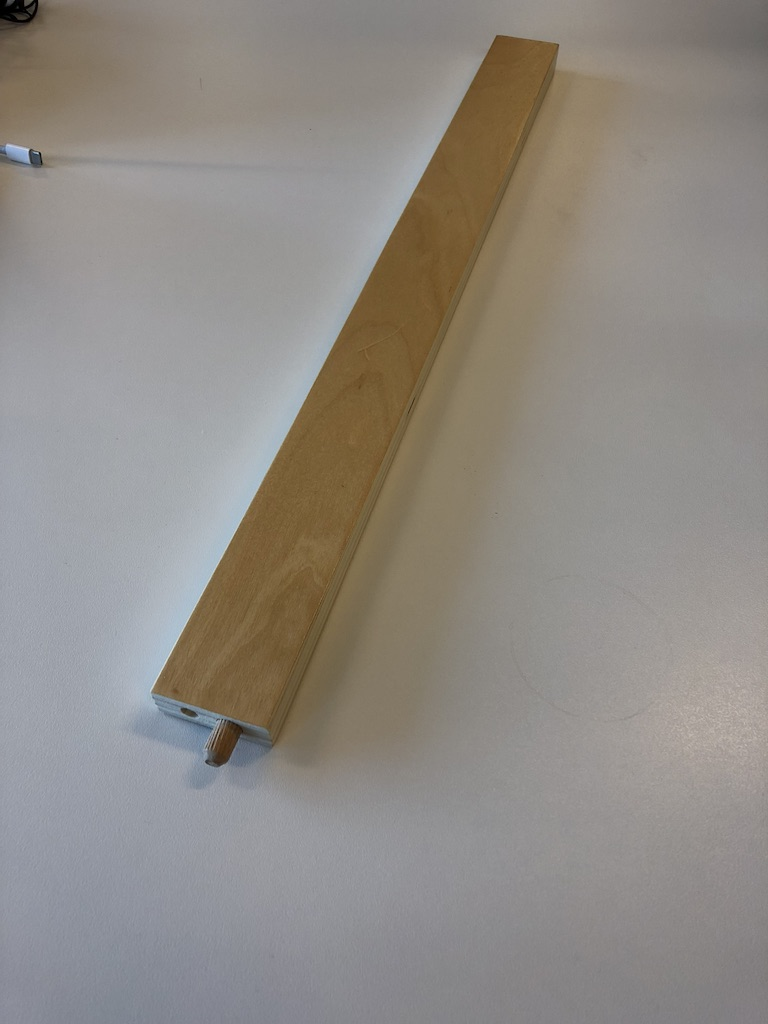
\includegraphics[width = 0.5\textwidth]{./Images/im1.jpg} 
\caption{Example image}
\end{center}
\end{figure}

\newpage

\begin{center}
\textbf{Log book}
\end{center}

\textbf{2018-09-18}
When training the object recognition net, they where trained on only the red channel and although it technically worked by inputting an RGB image later on, it obviously gave us completely bogus results.